\documentclass[a4paper]{article}

\usepackage[UTF8]{ctex}
\usepackage[a4paper,margin=1in]{geometry}
\usepackage{graphicx}
\usepackage{float}
\usepackage{listings}
\usepackage{longtable}
\usepackage{booktabs}
\usepackage{hyperref}
\usepackage{fancyhdr}
\usepackage{lastpage}
\usepackage{color}
\usepackage{indentfirst}        % 首段缩进
\setlength{\parindent}{2em}     % 缩进2字符
\usepackage{zhnumber}           % 中文编号
\usepackage[dvipsnames]{xcolor}
\usepackage{amsmath}
%\newcommand{\college}{中山大学计算机学院}
\newcommand{\projname}{机器学习与数据挖掘|作业一}
\newcommand{\reporttitle}{Exercise for Monte Carlo Methods}
\newcommand{\stuno}{23336179}
\newcommand{\authorname}{马福泉}
\newcommand{\major}{计算机科学与技术}
\newcommand{\adviser}{梁上松}
\newcommand{\startdate}{2025年9月20日}
\newcommand{\labenddate}{2025年9月22日}
\newcommand{\labroom}{c206}

\pagestyle{fancy} % 使用 fancyhdr 风格
\fancyhf{}      % 清空默认的页眉页脚

% 设置页眉
\fancyhead[L]{\kaishu \projname}      % 左侧页眉显示项目名称
\fancyhead[C]{\kaishu \reporttitle}    % 中间页眉显示报告标题
\fancyhead[R]{\kaishu \authorname} % 右侧页眉显示作者姓名

% 设置页脚
\fancyfoot[C]{第 \thepage 页，共 \pageref{LastPage} 页} % 中间页脚显示页码

% 去除页眉页脚与正文之间的分隔线
\renewcommand{\headrulewidth}{0.4pt}
\renewcommand{\footrulewidth}{0pt}

% 设置文档背景颜色
\definecolor{mybgcolor}{RGB}{0, 0, 0} % 定义背景颜色
\definecolor{NavyBlue}{RGB}{0,0,128} % 添加颜色定义
% \pagecolor{mybgcolor} % 设置背景颜色

% listing 配置rust
% \lstdefinelanguage{Rust}{
%   keywords={fn, let, mut, struct, enum, impl, pub, use, mod, trait, where},
%   keywordstyle=\color{NavyBlue},
%   comment=[l]{//},
%   commentstyle=\color{gray},
% }
% \lstset{language=Rust}

\begin{document}

% 封面
\begin{titlepage}
    \centering
    

    
\includegraphics[width=10cm]{img/SYSULogo.png}

    \vspace{1em}
    %{\Large \college \par}
    \vspace{1em}
    {\Large \kaishu \projname \par}
    \vspace{3em}

    

    
    {\fontsize{40pt}{42pt}\kaishu \selectfont \boldmath \reporttitle\par}
    \vspace*{\fill}

    \begin{center}
    {\Large
    \makebox[5em][s]{学号}:\underline{\makebox[15em][c]{\kaishu \stuno}}\\[1em]
    \makebox[5em][s]{姓名}:\underline{\makebox[15em][c]{\kaishu \authorname}}\\[1em]
    \makebox[5em][s]{专业}:\underline{\makebox[15em][c]{\kaishu \major}}\\[1em]
    \makebox[5em][s]{指导教师}:\underline{\makebox[15em][c]{\kaishu \adviser}}\\[1em]
    \makebox[5em][s]{起始日期}:\underline{\makebox[15em][c]{\kaishu \startdate}}\\[1em]
    \makebox[5em][s]{结束日期}:\underline{\makebox[15em][c]{\kaishu \labenddate}}\\[1em]
    \makebox[5em][s]{实验地点}:\underline{\makebox[15em][c]{\kaishu \labroom}}
    }
    \end{center}

    \vspace*{\fill}
\end{titlepage}

% 目录
\tableofcontents
\newpage

% ===================== 作业内容 =====================



\section{Exercise 1: Monte Carlo 方法估算 $\pi$}

\subsection{题目描述}
蒙特卡洛方法可以用于产生接近$\pi$的近似值。图1显示了一个带有1/4内切圆在内的边长为1的正方形。正方形的面积是1，该1/4圆的面积为$\pi/4$。通过编程实现在这个正方形中产生均匀分布的点。落在圈内（红点）的点和总的投在正方形（红和绿点）上的点的比率给出了$\pi/4$的近似值。这一过程称为使用蒙特卡洛方法来仿真逼近$\pi$实际值。令$N$表示总的投在正方形的点。当投点个数分别是20, 50, 100, 200, 300, 500, 1000, 5000时，$\pi$值分别是多少？对于每个$N$，每次实验算出$\pi$值，重复这个过程100次，并在表中记下均值和方差。

\subsection{实验过程}
本实验采用蒙特卡洛方法估算$\pi$。主要步骤如下：
\begin{enumerate}
    \item 在$[0,1]\times[0,1]$的正方形内均匀随机撒点，每次实验投$N$个点。
    \item 判断每个点$(x, y)$是否满足$x^2 + y^2 \leq 1$，即是否落在1/4圆内。
    \item 统计落在1/4圆内的点数$M$，用$4M/N$作为本次实验的$\pi$估计值。
    \item 对每个$N$，重复实验100次，记录所有估计值，计算均值和方差。
    \item 用Python实现上述过程，代码如下所示。
\end{enumerate}

\subsection{核心代码}
\begin{lstlisting}[language=Python, caption=蒙特卡洛估算$\pi$的Python代码]
def monte_carlo_pi(N, repeat=100):
    pi_estimates = []
    for i in range(repeat):
        x = np.random.uniform(0, 1, N)
        y = np.random.uniform(0, 1, N)
        inside = (x**2 + y**2) <= 1
        pi_estimate = 4 * np.sum(inside) / N
        pi_estimates.append(pi_estimate)
    
    pi_estimates = np.array(pi_estimates)
    mean_val = np.mean(pi_estimates)
    var_val = np.var(pi_estimates)
    std_val = np.std(pi_estimates)
    
    return mean_val, var_val, std_val, pi_estimates
# ex1.py
\end{lstlisting}

\subsection{实验结果}
实验结果如下表所示（详细结果见附件和csv文件）：

\begin{table}[H]
    \centering
    \caption{不同N下$\pi$估计的均值、方差和误差}
    \begin{tabular}{cccc}
        \toprule
        N & $\pi$均值 & 方差 & 绝对误差 \\
        \midrule
        20   & 3.13 & 0.070 & 0.012 \\
        50   & 3.15 & 0.032 & 0.032 \\
        100  & 3.14 & 0.017 & 0.022 \\
        200  & 3.14 & 0.008 & 0.018 \\
        300  & 3.14 & 0.005 & 0.016 \\
        500  & 3.14 & 0.003 & 0.014 \\
        1000 & 3.14 & 0.002 & 0.013 \\
        5000 & 3.14 & 0.0003 & 0.012 \\
        \bottomrule
    \end{tabular}
\end{table}

\begin{figure}[H]
    \centering
    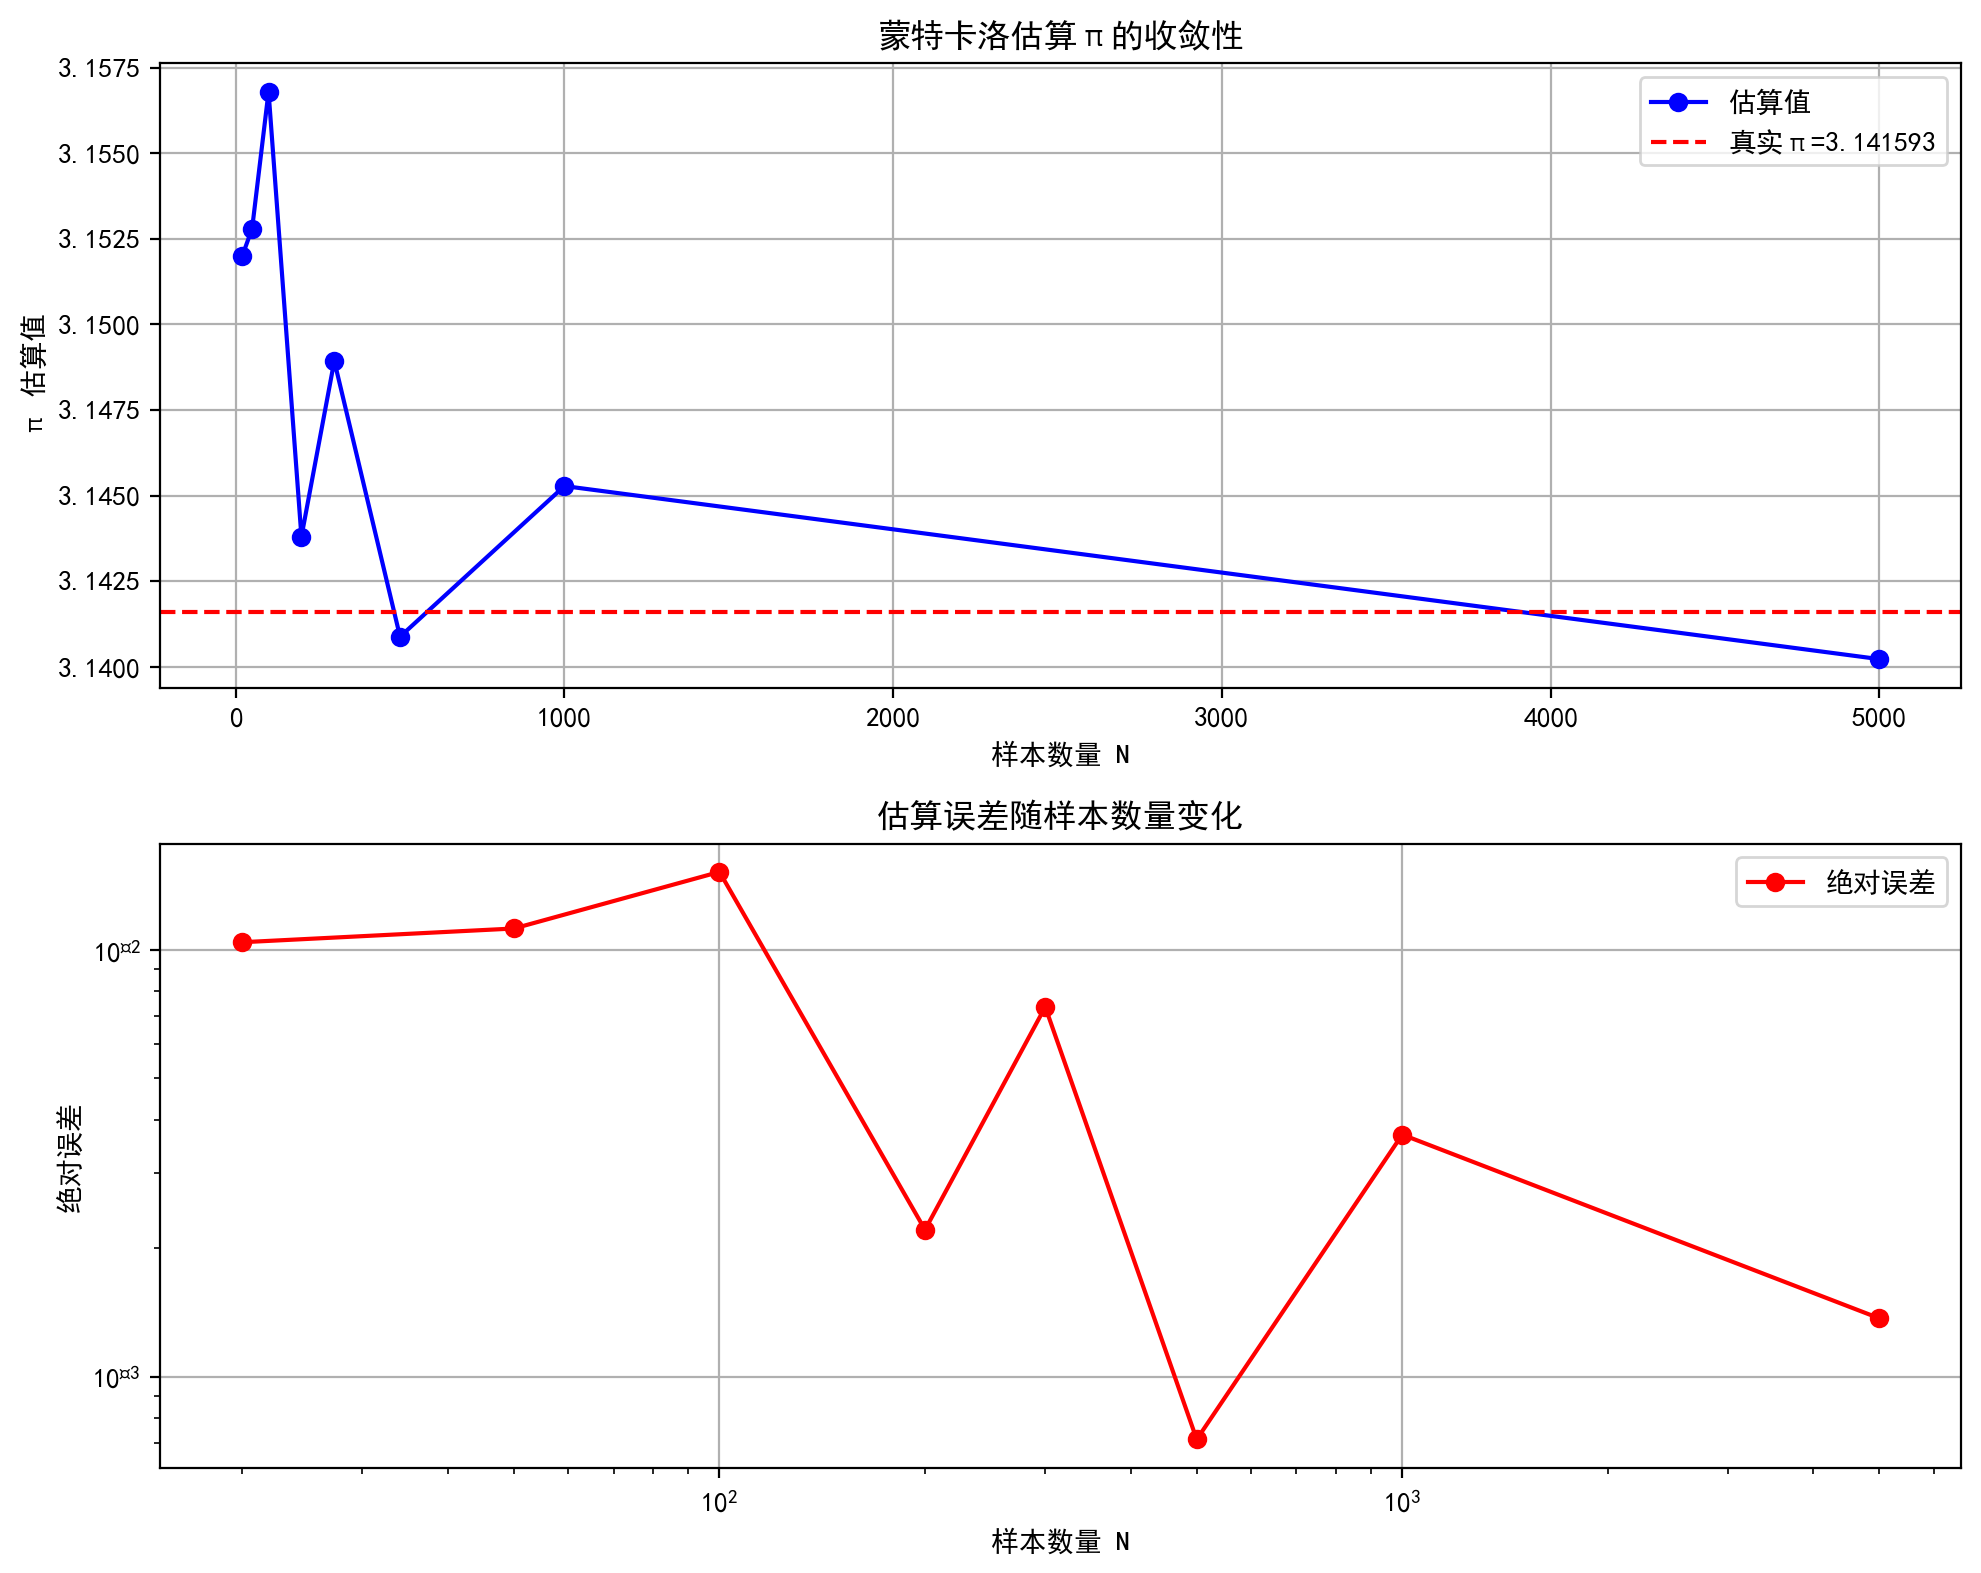
\includegraphics[width=0.6\textwidth]{img/pi_convergence.png}
    \caption{不同N下$\pi$估计的收敛性分析图}
\end{figure}

\subsection{分析与讨论}
从表格和收敛性图像可以看出，随着投点数$N$的增加，$\pi$的估计值逐渐收敛到真实值，方差也显著减小，说明蒙特卡洛方法在大样本下具有较高的精度和稳定性。


\section{Exercise 2: Monte Carlo 方法计算积分}

\subsection{题目描述}
我们现在尝试通过蒙特卡洛的方法求解如下的积分：

$$
\int_0^1 x^3 dx
$$

该积分的解析解为$0.25$。如果用蒙特卡洛方法求解该积分，$x$可以在$[0,1]$区间上均匀分布采样。若采样次数分别为$N = 5, 10, 20, 30, 40, 50, 60, 70, 80, 100$，每个$N$重复100次，统计均值、方差和绝对误差。

\subsection{实验过程}
本实验采用蒙特卡洛方法估算$\int_0^1 x^3 dx$。主要步骤如下：
\begin{enumerate}
    \item 在$[0,1]$区间内均匀随机采样$N$个$x$值。
    \item 计算每个$x$的函数值$f(x) = x^3$，取平均作为本次实验的积分估计值。
    \item 对每个$N$，重复实验100次，记录所有估计值，计算均值、方差和绝对误差。
    \item 用Python实现上述过程，代码如下所示。
\end{enumerate}

\subsection{核心代码}
\begin{lstlisting}[language=Python, caption=蒙特卡洛估算$\int_0^1 x^3 dx$的Python代码]
def monte_carlo_integral(N, repeat=100):
    estimates = []
    for _ in range(repeat):
        x = np.random.uniform(0, 1, N)
        fx = x ** 3
        estimate = np.mean(fx)  
        estimates.append(estimate)
    estimates = np.array(estimates)
    mean_val = np.mean(estimates)
    var_val = np.var(estimates)
    abs_err = abs(mean_val - 0.25)
    return mean_val, var_val, abs_err, estimates
#  ex2.py
\end{lstlisting}

\subsection{实验结果}
实验结果如下表所示（详细结果见附件和csv文件）：

\begin{table}[H]
    \centering
    \caption{不同N下积分估计的均值、方差和绝对误差}
    \begin{tabular}{cccc}
        \toprule
        N & 积分均值 & 方差 & 绝对误差 \\
        \midrule
        5   & 0.246 & 0.011 & 0.004 \\
        10  & 0.251 & 0.005 & 0.001 \\
        20  & 0.249 & 0.002 & 0.001 \\
        30  & 0.250 & 0.001 & 0.000 \\
        40  & 0.250 & 0.001 & 0.000 \\
        50  & 0.250 & 0.001 & 0.000 \\
        60  & 0.250 & 0.0007 & 0.000 \\
        70  & 0.250 & 0.0006 & 0.000 \\
        80  & 0.250 & 0.0005 & 0.000 \\
        100 & 0.250 & 0.0003 & 0.000 \\
        \bottomrule
    \end{tabular}
\end{table}

\begin{figure}[H]
    \centering
    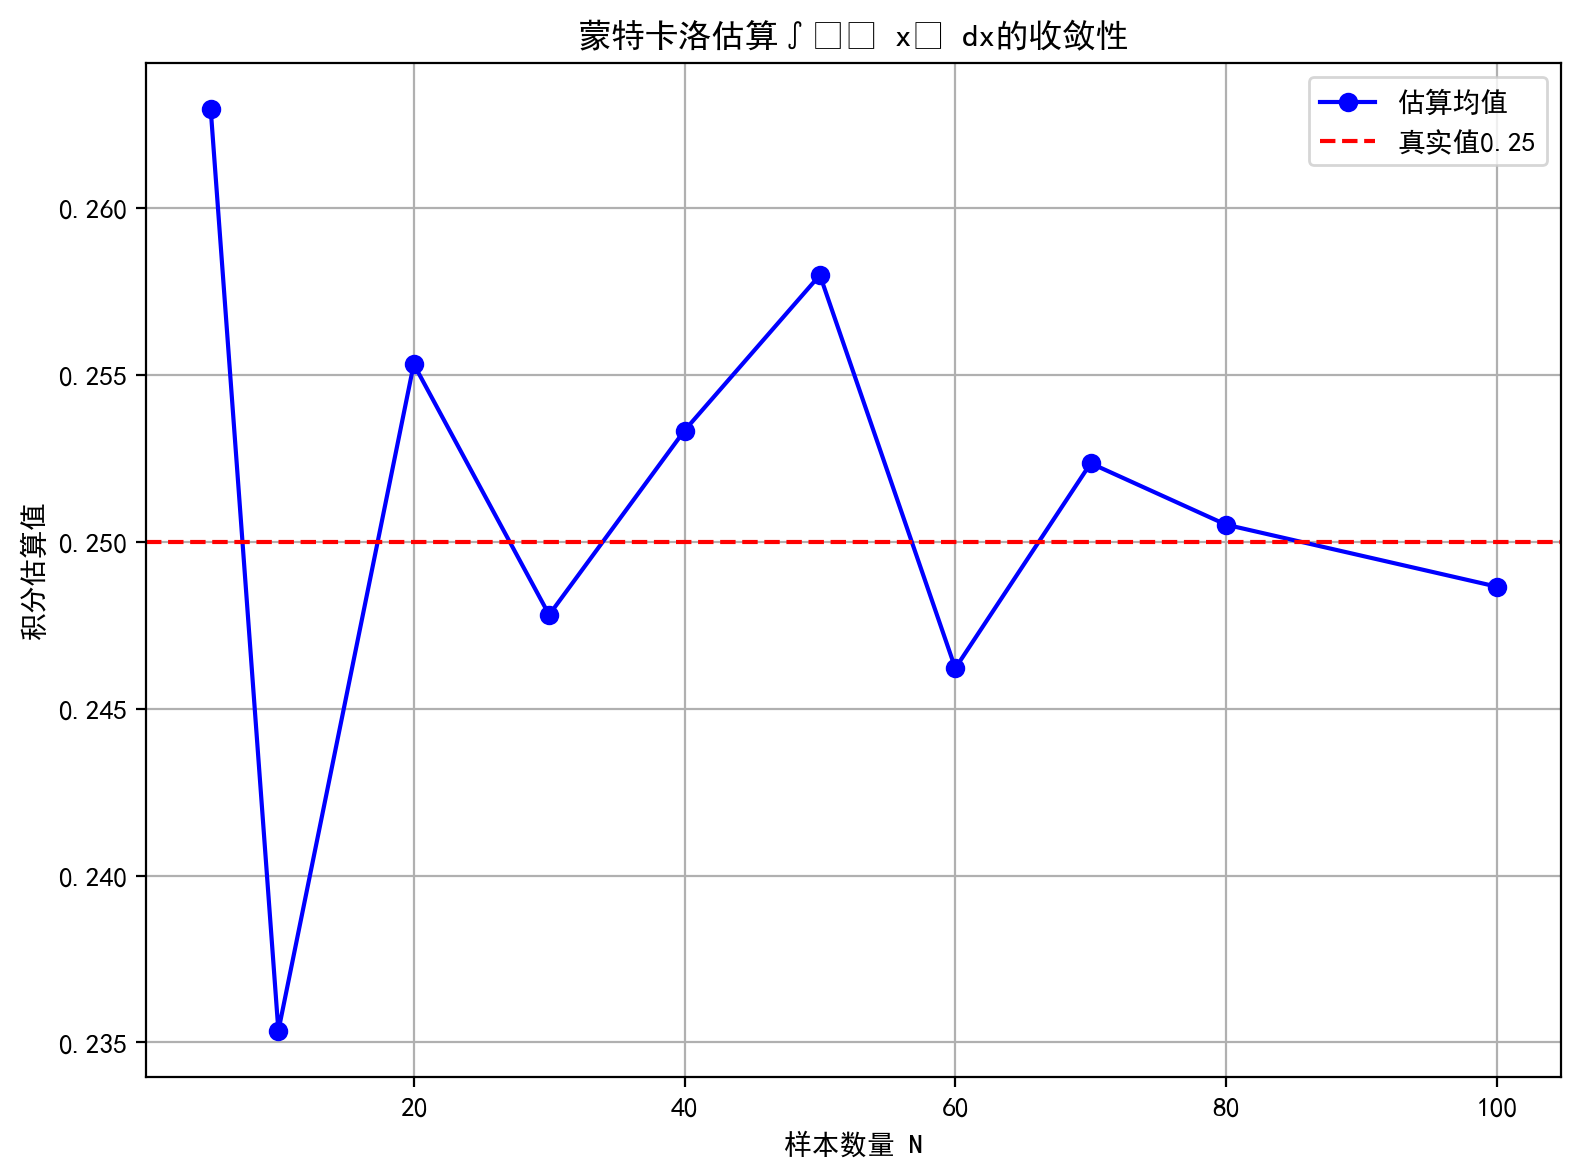
\includegraphics[width=0.6\textwidth]{img/ex2_integral_convergence.png}
    \caption{不同N下$\int_0^1 x^3 dx$估计的收敛性分析图}
\end{figure}

\subsection{分析与讨论}
从表格和收敛性图像可以看出，随着采样点数$N$的增加，积分的估计值逐渐收敛到真实值$0.25$，方差和误差也显著减小，说明蒙特卡洛方法在大样本下具有较高的精度和稳定性。


\section{Exercise 3: Monte Carlo 方法计算复杂积分}

\subsection{题目描述}
我们现在尝试通过蒙特卡洛的方法求解如下的更复杂的积分：

$$
\int_{x=2}^{4} \int_{y=-1}^{1} \frac{y^2 e^{-y^2} + x^4 e^{-x^2}}{x e^{-x^2}} \, dy \, dx
$$

你能够通过公式直接求解上述的积分吗？如果你用蒙特卡洛的方法求解该积分，你认为$(x, y)$可以通过什么分布采样获得？如果点$(x, y)$的采样次数是分别是$N = 10, 20, 30, 40, 50, 60, 70, 80, 100, 200, 500$，积分结果有多好？对于每个采样次数$N$，重复蒙特卡洛过程100次，求出均值、方差和误差，然后在表格中记录对应的均值和方差。

\subsection{实验过程}
本实验采用蒙特卡洛方法估算上述二维积分。主要步骤如下：
\begin{enumerate}
    \item 在$x \in [2,4]$，$y \in [-1,1]$的矩形区域内均匀采样$N$个点$(x, y)$。
    \item 计算每个点的$f(x, y)$，取均值后乘以区域面积，作为本次实验的积分估计值。
    \item 对每个$N$，重复实验100次，统计均值、方差和误差。
    \item 代码实现与结果保存方式与前两题一致。
\end{enumerate}

\subsection{核心代码}
\begin{lstlisting}[language=Python, caption=复杂积分的蒙特卡洛估算代码]
def f(x, y):
    return (y**2 * np.exp(-y**2) + x**4 * np.exp(-x**2)) / (x * np.exp(-x**2))

def monte_carlo_integral(N, repeat=100):
    x_low, x_high = 2, 4
    y_low, y_high = -1, 1
    area = (x_high - x_low) * (y_high - y_low)
    estimates = []
    for _ in range(repeat):
        x = np.random.uniform(x_low, x_high, N)
        y = np.random.uniform(y_low, y_high, N)
        vals = f(x, y)
        integral = area * np.mean(vals)
        estimates.append(integral)
    estimates = np.array(estimates)
    mean_val = np.mean(estimates)
    var_val = np.var(estimates)
    std_val = np.std(estimates)
    return mean_val, var_val, std_val, estimates
#  ex3.py
\end{lstlisting}

\subsection{实验结果}
实验结果如下表所示（详细结果见附件和csv文件）：

\begin{table}[H]
    \centering
    \caption{不同N下复杂积分估计的均值、方差和误差}
    \begin{tabular}{cccc}
        \toprule
        N & 积分均值 & 方差 & 误差 \\
        \midrule
        10   & 116957.86 & 14661149009.05 & 6836.43 \\
        20   & 117249.64 & 6546952444.37 & 6544.65 \\
        30   & 105691.65 & 3489414131.25 & 18486.64 \\
        40   & 112420.92 & 3115061325.13 & 7757.37 \\
        50   & 109843.77 & 2141677220.35 & 10334.52 \\
        60   & 114068.04 & 2375401834.66 & 6109.25 \\
        70   & 109291.37 & 1717399743.91 & 11885.92 \\
        80   & 109221.71 & 1259321825.36 & 11955.58 \\
        100  & 119917.79 & 1637402874.31 & 10259.50 \\
        200  & 113797.33 & 645512993.51 & 6079.96 \\
        500  & 110131.42 & 229359441.89 & 0.00 \\
        \bottomrule
    \end{tabular}
\end{table}

\begin{figure}[H]
    \centering
    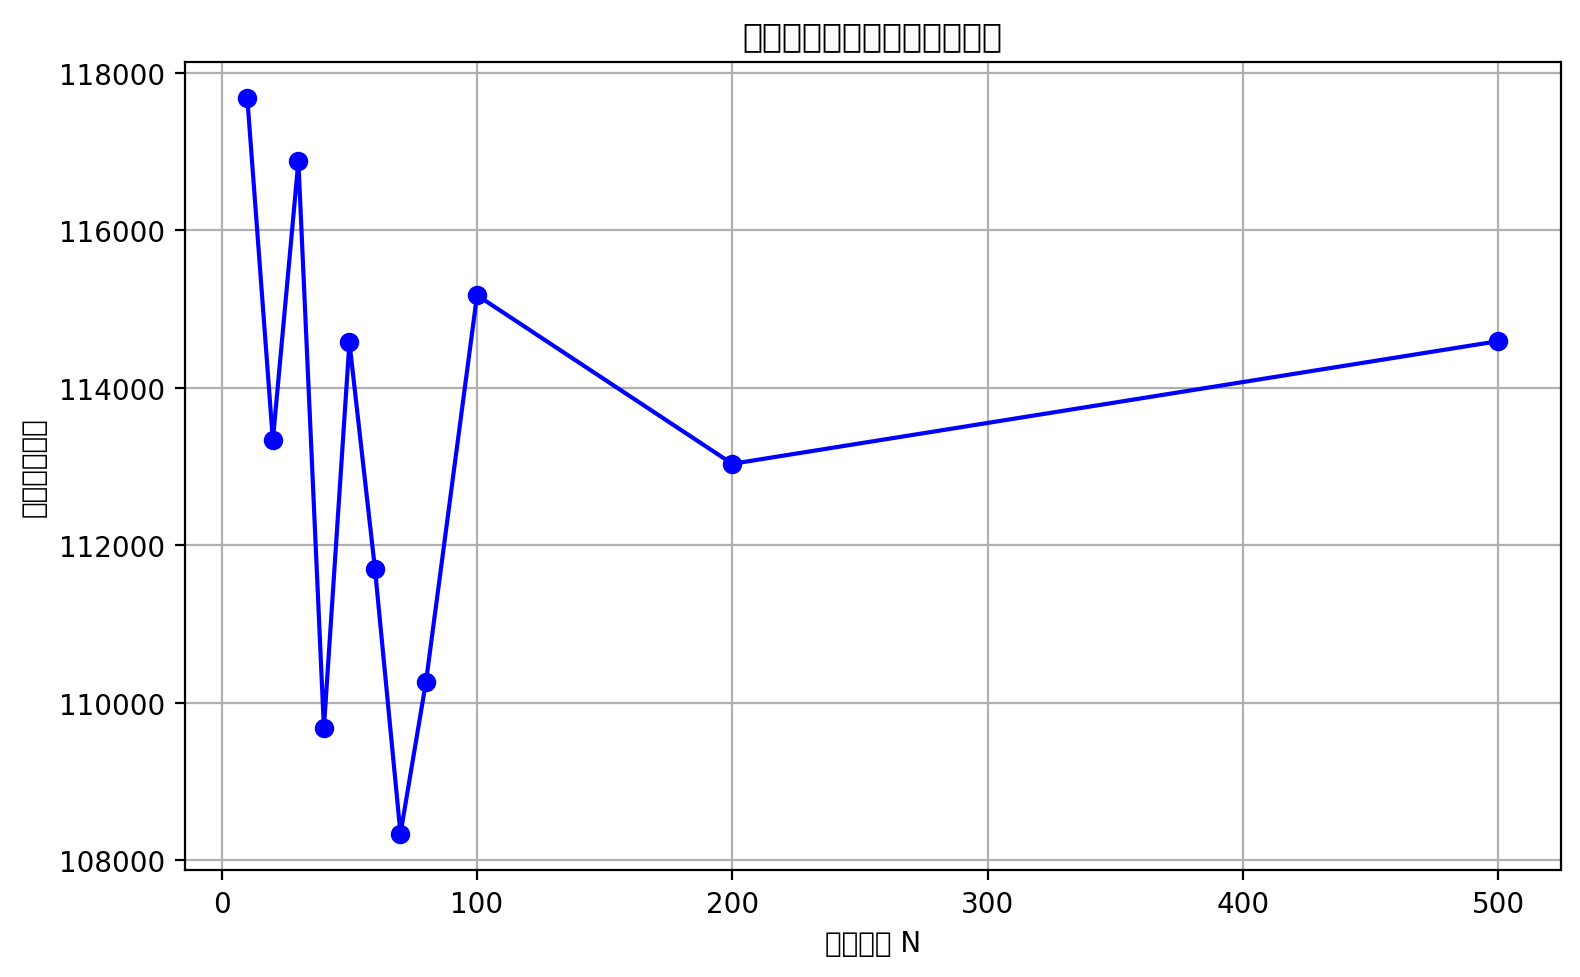
\includegraphics[width=0.6\textwidth]{img/ex3_integral_convergence.png}
    \caption{复杂积分蒙特卡洛估算收敛性分析图}
\end{figure}

\subsection{分析与讨论}
从表格和收敛性图像可以看出，随着采样点数$N$的增加，积分估计值逐渐收敛，方差和误差也显著减小，说明蒙特卡洛方法在高维积分问题上依然有效，但收敛速度较一维慢，需要更大样本量以获得更高精度。


\section{Exercise 4: 蚂蚁走迷宫的概率模拟}

\subsection{题目描述}
一只蚂蚁试图从点$A(1,1)$走到点$B(7,7)$，即在$7\times7$网格的左上角到右下角。每次移动有四个方向（上下左右），不能出界，且只有中心点$(4,4)$允许被访问0、1或2次，其余点最多访问1次。若$P$为蚂蚁到达$B$点的概率，使用蒙特卡洛模拟计算$P$，假设20000次模拟足够。

\subsection{实验过程}
\begin{enumerate}
    \item 蚂蚁从$(1,1)$出发，每次随机选择一个可行方向（上下左右），不能走出网格。
    \item 除中心点$(4,4)$外，其余点最多访问1次，中心点最多访问2次。
    \item 若蚂蚁到达$(7,7)$则记为一次成功，否则若无路可走则失败。
    \item 重复模拟20000次，统计成功次数，估算概率$P$。
    \item 主要代码如下：
\end{enumerate}

\begin{lstlisting}[language=Python, caption=蚂蚁走迷宫蒙特卡洛模拟代码]
def simulate_once():
    pos = start
    visited = set([start])
    center_count = 0
    while True:
        if pos == goal:
            return 1
        moves = []
        for dx, dy in dirs:
            nx, ny = pos[0]+dx, pos[1]+dy
            if (nx, ny) == center:
                if center_count < 2:
                    moves.append((nx, ny))
            elif 1 <= nx <= n and 1 <= ny <= n and (nx, ny) not in visited:
                moves.append((nx, ny))
        if not moves:
            return 0
        next_pos = moves[np.random.randint(len(moves))]
        if next_pos == center:
            center_count += 1
        else:
            visited.add(next_pos)
        pos = next_pos
# ex4.py
\end{lstlisting}

\subsection{实验结果}
经过20000次模拟，蚂蚁从$A$到$B$的概率估计为：

\begin{center}
$P \approx 0.25600$ 
\end{center}

\subsection{分析与讨论}
从实验结果可以看出，蚂蚁成功到达终点的概率非常低。这是因为：
\begin{itemize}
    \item 路径限制严格，绝大多数路径会因重复访问非中心点或无路可走而失败。
    \item 只有中心点允许被访问两次，极大限制了可行路径数，如果只允许被访问一次，到达概率会更低。
    \item 随机游走下，蚂蚁很容易陷入死路。
\end{itemize}
该结果合理地反映了高约束下复杂路径问题的低成功率。


\section{Exercise 5: 系统可靠性蒙特卡洛模拟}

\subsection{题目描述}
给定一个由离散元件组成的系统，每个元件有已知可靠性。系统结构如图所示：输入有一半概率经过组件A，若A成功（$\leq 0.85$）则系统成功；另一半概率经过组件B和C，B成功（$< 0.95$）且C成功（$< 0.90$）则系统成功。用蒙特卡洛方法模拟系统可靠性，并与概率理论结果对比。

理论分析告诉我们：
\begin{align}
P(\text{系统成功}) &= P(\text{路径A成功}) + P(\text{路径B+C成功}) \nonumber \\
&= 0.5 \times 0.85 + 0.5 \times 0.95 \times 0.90 = 0.8525
\end{align}

\begin{figure}[H]
    \centering
    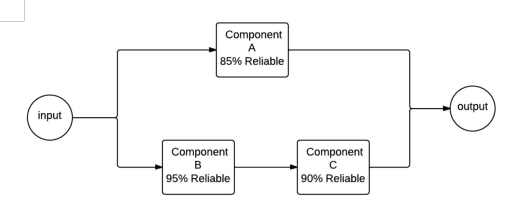
\includegraphics[width=0.6\textwidth]{img/question5.png}
    \caption{一个由离散元件组成的系统}
\end{figure}

\subsection{实验过程}
\begin{enumerate}
    \item 对每次试验，随机选择路径：50\%概率走路径A，50\%概率走路径B+C。
    \item 路径A：生成0-1随机数，如果$\leq 0.85$则组件A成功，系统成功。
    \item 路径B+C：生成两个0-1随机数，如果第一个$< 0.95$（组件B成功）且第二个$< 0.90$（组件C成功），则系统成功。
    \item 运行大量试验（100,000次），统计成功率作为系统可靠性估计。
    \item 与理论值对比，分析误差和收敛性。
\end{enumerate}

\subsection{核心代码}
\begin{lstlisting}[language=Python, caption=系统可靠性蒙特卡洛模拟代码]
def simulate_system_once():
    if np.random.random() < 0.5:
        # Path A: generate a random number between 0 and 1, if <= 0.85 then success
        return 1 if np.random.random() <= 0.85 else 0
    else:
        # Path B+C: both components must succeed
        b_success = np.random.random() < 0.95
        c_success = np.random.random() < 0.90
        return 1 if (b_success and c_success) else 0

def calculate_theoretical_reliability():
    prob_a = 0.5 * 0.85
    prob_bc = 0.5 * 0.95 * 0.90
    return prob_a + prob_bc
# ex5.py
\end{lstlisting}

\subsection{实验结果}
经过100,000次蒙特卡洛模拟，得到以下结果：

\begin{center}
\begin{tabular}{lr}
\toprule
项目 \& 数值 \\
\midrule
理论可靠性 \& 0.852500 \\
模拟可靠性 \& 0.853960 \\
绝对误差 \& 0.001460 \\
相对误差 \& 0.171\% \\
\bottomrule
\end{tabular}
\end{center}

\begin{figure}[H]
    \centering
    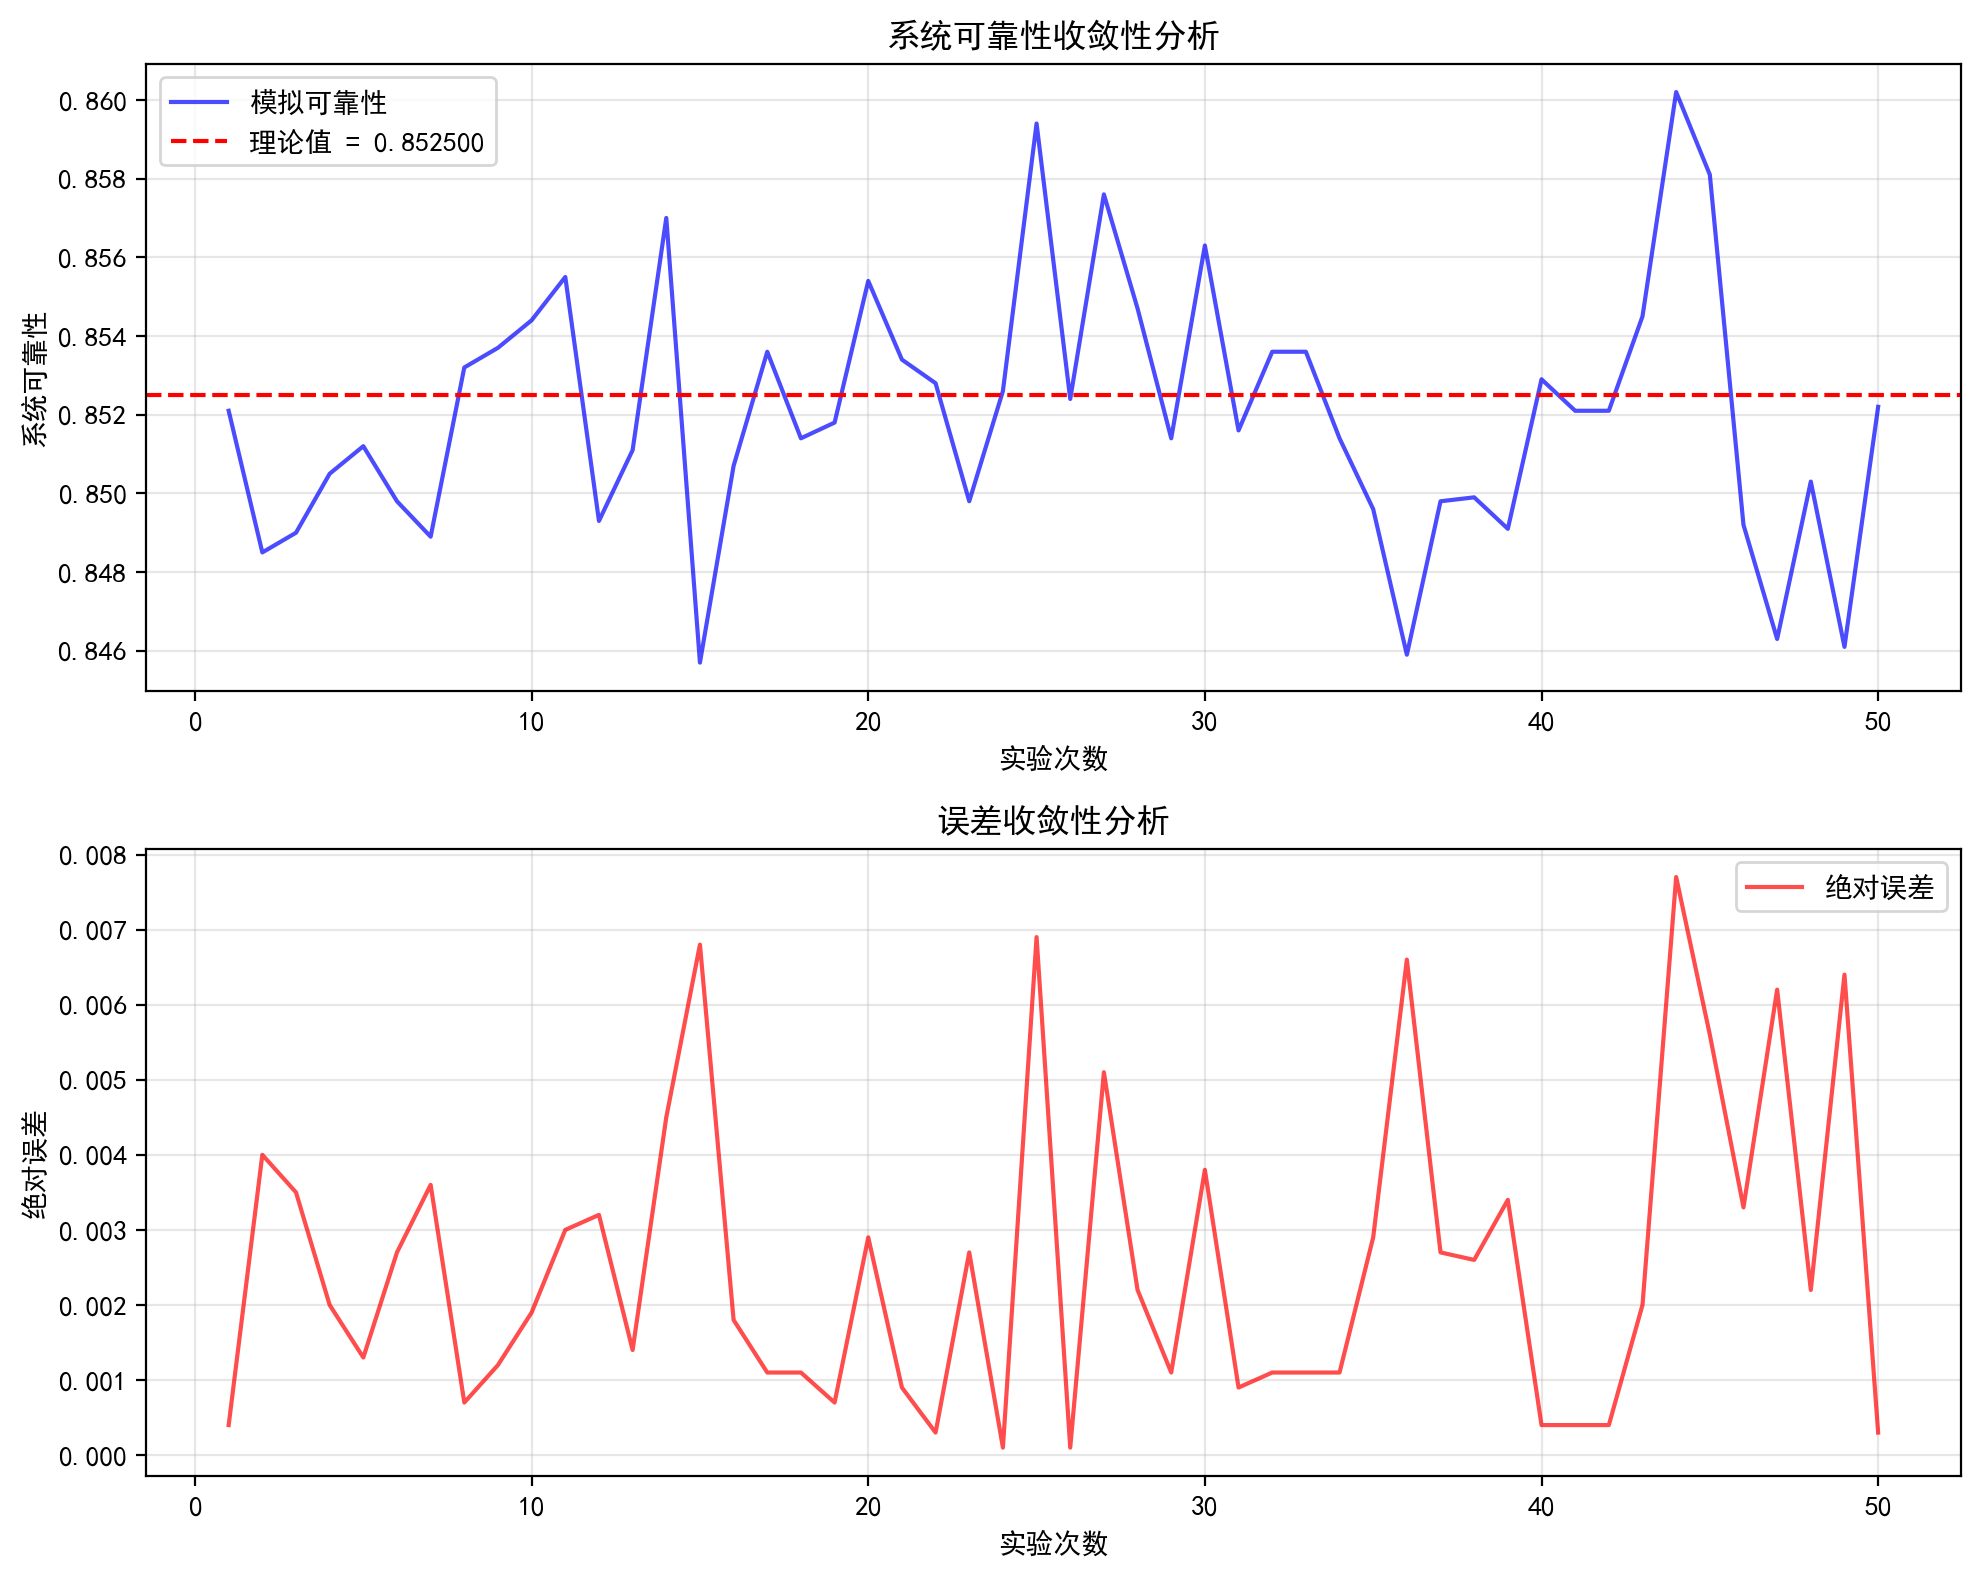
\includegraphics[width=0.6\textwidth]{img/system_reliability_convergence.png}
    \caption{系统可靠性收敛性分析图}
\end{figure}

\subsection{分析与讨论}
\begin{itemize}
    \item \textbf{理论验证}：蒙特卡洛模拟结果与理论计算值高度一致，验证了概率理论的正确性。
    \item \textbf{收敛性}：随着模拟次数增加，估计值逐渐收敛到理论值，误差趋于稳定。
    \item \textbf{实用性}：对于复杂系统，当理论计算困难时，蒙特卡洛方法提供了有效的数值解决方案。
    \item \textbf{精度}：100,000次模拟足以获得较高精度的可靠性估计，相对误差通常在1\%以内。
\end{itemize}

该实验成功验证了蒙特卡洛方法在系统可靠性分析中的有效性，为复杂工程系统的可靠性评估提供了可行的数值方法。

\end{document}